\documentclass{article}

\usepackage[final]{neurips}
\usepackage[utf8]{inputenc}
\usepackage[T1]{fontenc}
\usepackage[spanish,es-noquoting]{babel}
% babel-spanish pone coma decimal SOLO en modo matematico, asi que el documento
% mezclaba «IoU 0.681» (texto) con «$+0,135$» (matematico) en la misma frase.
% Se unifica en punto, que es lo que usan los numeros en texto, que son mayoria.
\decimalpoint
\usepackage{hyperref}
\usepackage{url}
\usepackage{booktabs}
\usepackage{amsfonts}
\usepackage{amsmath}
\usepackage{nicefrac}
\usepackage{microtype}
\usepackage{graphicx}
\usepackage{float}
\usepackage{natbib}
% neurips.sty fija el titulo de la bibliografia en "References"; se traduce aqui.
\renewcommand{\bibsection}{\section*{\normalsize\bfseries Referencias}}

% --- Ubicacion de flotantes -------------------------------------------
% Mas margen para que las tablas compartan pagina con el texto en vez de
% irse solas y dejar media pagina en blanco. No cambia margenes ni fuente.
\renewcommand{\topfraction}{0.95}
\renewcommand{\bottomfraction}{0.9}
\renewcommand{\textfraction}{0.06}
\renewcommand{\floatpagefraction}{0.85}
% Con ocho flotantes, la separacion por defecto (~20 pt arriba y abajo de cada
% uno) suma casi un cuarto de pagina de blanco. Se reduce sin tocar margenes ni
% cuerpo de letra, que es lo que el enunciado fija.
\setlength{\textfloatsep}{11pt plus 2pt minus 2pt}
\setlength{\floatsep}{9pt plus 2pt minus 2pt}
\setlength{\intextsep}{9pt plus 2pt minus 2pt}
\setcounter{totalnumber}{4}

\title{Segmentación de inundaciones en Sentinel-1 con U-Net:\\
       supervisión débil, generalización geográfica y fusión con Sentinel-2}

\author{%
  Flavio César Amayo Gamboa \quad Gustavo Adolfo Huarcaya Delgado \\
  Jhordy Joel Maximiliano Cusi \quad Sergio Mondragon Contreras \\
  Facultad de Ingeniería Industrial y de Sistemas \\
  Universidad Nacional de Ingeniería
}

\date{31 de octubre de 2026}

\begin{document}

\maketitle

\begin{abstract}
Se implementa una U-Net desde cero en PyTorch para segmentar agua de inundación
en imágenes SAR de Sentinel-1 sobre Sen1Floods11. Dentro de distribución el
modelo alcanza IoU 0.681 y supera a la umbralización de Otsu por $+0.135$, con
intervalo de confianza que no cruza cero. En la región geográfica retenida,
Bolivia, el orden se invierte: Otsu gana por $+0.088$, también de forma
significativa. Los resultados principales son cuatro.
Primero, agregar los chips de etiqueta débil empeora la IoU de 0.681 a 0.587:
llevan el entrenamiento a 4\,412 chips, diecisiete veces más datos. Segundo, el
análisis de fallos muestra que el 99.8\% de los falsos positivos y el 96.5\% de
los negativos se concentran donde VV no separa agua de suelo: las densidades de
retrodispersión de agua y suelo se solapan un 41.2\%, y los errores del modelo
caen en esa zona. Tercero, fusionar Sentinel-2 sube la IoU a 0.850 ($+0.169$,
significativo), pero la fusión no le gana al óptico solo; el radar solo vuelve a
pesar bajo nube, donde con 16 chips nublados la diferencia no se puede afirmar.
Cuarto, sobre la
región peruana construida para este trabajo el modelo cae a IoU 0.003, pero la
causa no es falta de generalización: la etiqueta oficial de Copernicus marca la
extensión máxima de la inundación y no la superficie de agua visible en SAR, y su
retrodispersión mediana ($-9.2$
dB) se parece al suelo de Sen1Floods11 ($-8.4$) y no a su agua ($-16.5$).
\end{abstract}

% ============================================================================
\section{Motivación}
% ============================================================================

Durante una inundación, saber \emph{dónde} está el agua en las horas siguientes
decide a dónde se manda la ayuda. El satélite óptico es la herramienta natural
para mirar el terreno, pero las nubes que acompañan a la tormenta lo dejan ciego
justo cuando más se lo necesita. El radar de apertura sintética de Sentinel-1
\citep{torres2012sentinel1} atraviesa la nube y adquiere de noche, lo que lo
convierte en la herramienta de facto para el mapeo rápido de inundaciones.

El problema tiene un precedente peruano concreto: durante las inundaciones de
Lima de marzo de 2017 (El Niño costero) el Servicio de Gestión de
Emergencias de Copernicus activó el mapeo rápido EMSN038
\citep{copernicus2017emsn038} para delinear la extensión del agua en Carapongo,
Comas, Puente de Piedra y otros distritos de los ríos Rímac y Chillón.

El reto no es solo arquitectónico. No todas las etiquetas del conjunto son igual
de confiables: Sen1Floods11 \citep{bonafilia2020sen1floods11} distingue entre 446
\emph{chips} anotados a mano por expertos y 4\,385 generados automáticamente por
umbralización, abundantes pero ruidosos. Decidir cómo combinar ambas fuentes es
parte del trabajo, y este informe sostiene que esa decisión importa más que
cualquier variante de la arquitectura.

% ============================================================================
\section{Trabajos relacionados}
% ============================================================================

\paragraph{Segmentación con codificador-decodificador.}
La U-Net \citep{ronneberger2015unet} introdujo la combinación de un camino
contractivo que gana contexto, uno expansivo que recupera resolución, y
conexiones de salto que devuelven al decodificador el detalle espacial que el
codificador perdió al submuestrear. Esa combinación sigue siendo la referencia
en segmentación con pocos datos anotados, que es el régimen de este
problema: 252 chips de entrenamiento. Variantes posteriores agregan compuertas
de atención sobre las conexiones de salto \citep{oktay2018attention} o las
anidan en varias escalas \citep{zhou2018unetpp}; aquí se implementa la
formulación original y se ablaciona la profundidad, por las razones de la
Sección~\ref{sec:ablacion}.

\paragraph{Detección de agua en SAR.}
El método clásico es umbralizar la retrodispersión: el agua, al ser una
superficie lisa, refleja el pulso lejos del satélite y aparece oscura. La
umbralización de Otsu \citep{otsu1979threshold} elige el corte que maximiza la
varianza entre las dos clases, recalculándolo para cada escena. Esa recalibración por escena explica su
ventaja fuera de distribución (Sección~\ref{sec:generalizacion}).
Sen1Floods11 usa Otsu para generar sus etiquetas débiles.

\paragraph{Pérdidas para clases desbalanceadas.}
El agua ocupa el 9.5\% de los píxeles etiquetados del conjunto de entrenamiento.
La entropía cruzada sola premia predecir ``no agua'' en todo; el coeficiente de
Dice \citep{milletari2016vnet} optimiza directamente el solape entre predicción
y verdad, y es insensible al tamaño del fondo. Acá se evalúan las dos y su
combinación (Sección~\ref{sec:ablacion}).

\paragraph{Índices ópticos de agua.}
Para el bono se usan dos índices normalizados clásicos: NDWI
\citep{mcfeeters1996ndwi}, que contrasta verde contra infrarrojo cercano, y
MNDWI \citep{xu2006mndwi}, que reemplaza el NIR por el SWIR y es más robusto en
zona urbana. Ambos se calculan sobre las bandas de Sentinel-2
\citep{drusch2012sentinel2} que Sen1Floods11 distribuye emparejadas con el SAR.

% ============================================================================
\section{Conjunto de datos}
% ============================================================================

Sen1Floods11 cubre 11 eventos de inundación en distintos países y biomas. Cada
chip es un GeoTIFF de $512\times512$ píxeles a 10 m de resolución, en EPSG:4326,
con dos bandas SAR (VV y VH, en decibelios) y su contraparte óptica de
Sentinel-2 de 13 bandas.

La etiqueta dorada tiene tres valores: \texttt{1} agua, \texttt{0} no agua y
\texttt{-1} sin dato. El $-1$ no es un detalle de formato: marca los
píxeles que el anotador no pudo etiquetar, y tratarlo como ``no agua'' inventaría
supervisión negativa donde no la hay. La pérdida de este trabajo lo enmascara
explícitamente (Sección~\ref{sec:perdida}).

\paragraph{Partición.} Se usa la oficial del conjunto: 252 chips de
entrenamiento, 89 de validación y 90 de prueba, más los 15 de Bolivia,
que los autores reservan como región geográfica independiente. Bolivia nunca se
ve durante el entrenamiento, ni siquiera a través de los chips débiles: el
conjunto débil incluye 224 chips bolivianos, y agregarlos ``porque vienen del
otro conjunto'' sería una fuga de información hacia la región de prueba.

\paragraph{Normalización, medida y congelada.} Las estadísticas se calculan
solo sobre los 252 chips de entrenamiento: VV tiene media $-10.39$ dB
con desvío $4.04$, y VH media $-17.24$ con desvío $4.75$. Los valores se recortan
a los percentiles 0.1 y 99.9 antes de estandarizar, porque el mínimo observado
($-65.45$ dB en VV) es un artefacto aislado que aplastaría todo el rango útil.
Calcular estas constantes sobre el conjunto completo filtraría información de
prueba en la normalización.

% ============================================================================
\section{Metodología}
% ============================================================================

\subsection{La U-Net, escrita desde cero}

El enunciado exige implementarla sin copiar código de bibliotecas de
segmentación existentes. La implementación tiene 31.04 M de parámetros y sigue
la formulación original: cuatro bloques de bajada, un cuello, cuatro de subida y
conexiones de salto por concatenación, no por suma, porque la suma obligaría
a que los dos tensores tengan la misma cantidad de canales y perdería la
distinción entre el detalle del codificador y el contexto del decodificador.

Decisiones de diseño:

El relleno es ``same'', no ``valid''. La U-Net original recorta en cada
convolución y su salida es más pequeña que la entrada. Aquí la salida mide
$512\times512$, porque la máscara está georreferenciada: un recorte
desplazaría la predicción respecto de las coordenadas del GeoTIFF y haría
imposible compararla píxel a píxel con la etiqueta.

La entrada son dos canales, VV y VH, no tres. Replicar a tres para
reusar pesos de ImageNet no tiene sentido aquí: no se parte de pesos
preentrenados, y la retrodispersión en decibelios no es una imagen RGB.

La salida son logits, no probabilidades. La sigmoide se aplica dentro
de la pérdida, que es numéricamente estable en su forma combinada.

\subsection{La pérdida enmascarada}
\label{sec:perdida}

La pérdida ignora los píxeles con etiqueta $-1$ multiplicando por una máscara
binaria antes de promediar. Hay un caso borde que importa: un lote donde
ningún píxel tiene etiqueta utilizable. Devolver
\texttt{torch.tensor(0.0)} ahí rompería el grafo de gradientes; se devuelve
\texttt{(logits * 0).sum()}, que es cero \emph{con} gradiente y deja el paso de
optimización bien definido.

\subsection{Cuatro decisiones del entrenamiento}

La época se elige por IoU de validación, no por pérdida. La pérdida
mezcla BCE y Dice y puede mejorar sin que la IoU se mueva; la métrica del
enunciado es la IoU, así que es la que decide qué pesos se guardan.

La aumentación son volteos y giros de 90 grados, nada más. Un recorte
aleatorio rompería la alineación con la grilla georreferenciada, y una rotación
que no sea múltiplo de 90 grados interpolaría la máscara e inventaría píxeles de
agua en los bordes.

Otsu se mide sobre los píxeles observados por ambos. El
conjunto trae \texttt{S1Otsu\allowbreak LabelHand} para esta
comparación; si Otsu se evaluara sobre todos los píxeles y la U-Net solo sobre
los etiquetados, no sería una comparación entre pares.

Bolivia se evalúa una sola vez, al final. Usarla para elegir
hiperparámetros la convertiría en una segunda validación y dejaría de medir
generalización.

\subsection{Protocolo de evaluación}

Se reportan dos IoU porque miden cosas distintas y el enunciado pide la
segunda. La \emph{agregada} suma los conteos de todos los chips y divide una vez:
pesa más los chips con mucha agua, y es la que se usa como principal porque pesa
cada píxel por igual y no se desestabiliza en los chips casi secos. La
\emph{promedio por chip}, la que usan los
autores del conjunto, da el mismo peso a cada chip y por eso es mucho más baja:
hay chips casi secos donde la IoU es inestable. Un chip sin un solo píxel de agua
ni predicho ni real tiene unión cero y se excluye del promedio, en vez de
contarlo como 0 o como 1.

Con 90 chips de prueba y 15 de Bolivia, una diferencia de IoU puede ser ruido de
muestreo, así que todas las comparaciones usan \emph{bootstrap}
\citep{efron1994bootstrap} pareado sobre chips, nunca sobre
píxeles: los píxeles vecinos de un chip están correlacionados (un río cubre
miles de píxeles que son una sola observación) y remuestrearlos daría
intervalos absurdamente angostos; las diferencias que no superan su intervalo se
declaran no afirmables en vez de reportarse.

% ============================================================================
\section{Experimentos y resultados}
% ============================================================================

\subsection{Evaluación en distribución (entregable 3)}

\begin{table}[!htbp]
\centering
\caption{Desempeño de la mejor configuración sobre las tres particiones. La
matriz de confusión es sobre píxeles observados, al umbral 0.5.}
\label{tab:distribucion}
\small
\begin{tabular}{lrrrrr@{\qquad}rrrr}
\toprule
& \multicolumn{5}{c}{Métricas} & \multicolumn{4}{c}{Confusión (px)} \\
\cmidrule(lr){2-6}\cmidrule(lr){7-10}
Conjunto & IoU & IoU/chip & $F_1$ & Precisión & Recall & VP & FP & FN & VN \\
\midrule
Validación (89) & 0.6521 & 0.4095 & 0.7894 & 0.8019 & 0.7773 & 1.74 M & 0.43 M & 0.50 M & 17.6 M \\
\textbf{Prueba (90)} & \textbf{0.6808} & 0.4178 & 0.8101 & 0.8111 & 0.8091 & 2.08 M & 0.48 M & 0.49 M & 17.5 M \\
Bolivia (15) & 0.6096 & 0.3758 & 0.7574 & 0.7849 & 0.7319 & 0.33 M & 0.09 M & 0.12 M & 2.32 M \\
\bottomrule
\end{tabular}
\end{table}

\paragraph{La matriz de confusión, comentada.}
La matriz está balanceada, y eso descarta que el umbral esté mal puesto. En
prueba hay 483\,649 falsos positivos contra 489\,788 falsos negativos, una
diferencia del 1.3\%, con precisión 0.811 y recall 0.809. Están balanceados, así
que mover el umbral de 0.5 no mejoraría la IoU: solo cambiaría un tipo de error
por el otro.
Eso obliga a buscar la causa del error en otra parte, que es lo que hace la
Sección~\ref{sec:fallos}.

La exactitud sería engañosa y por eso no se reporta como resultado. Los
verdaderos negativos son 17.5 M contra 2.08 M de verdaderos positivos: predecir
``no agua'' en todos los píxeles daría 88\% de exactitud sin segmentar nada. Por
eso la métrica del conjunto es la IoU de la clase agua, que ignora
los verdaderos negativos por construcción.

La brecha entre las dos IoU mide el desbalance entre chips. La
agregada es 0.6808 y la promedio por chip 0.4178, una diferencia de 0.26. Como la
agregada pesa cada píxel igual y la promedio pesa cada chip igual, esa brecha
dice que el modelo funciona bien en los chips con mucha agua y mal en los
casi secos. Los autores del
conjunto reportan la segunda, y por eso se reportan las dos.

De prueba a Bolivia el modelo cae en recall, no en precisión: la precisión
baja de 0.811 a 0.785 (un 3\%) mientras el recall cae de 0.809 a 0.732 (un 10\%).
El modelo no inventa más agua en terreno nuevo, deja de encontrarla. Es
consistente con la hipótesis de la recalibración por escena de la
Sección~\ref{sec:generalizacion}: un umbral aprendido en otras regiones queda
demasiado exigente cuando el histograma se corre.

\subsection{Estudio de ablación (entregable 2)}
\label{sec:ablacion}

\begin{table}[!htbp]
\centering
\caption{Las siete corridas de la ablación. Todas comparten semilla, partición y
presupuesto de cómputo (\textasciitilde10 minutos); las corridas con chips
débiles usan menos épocas porque cada época recorre más datos.}
\label{tab:ablacion}
\small
\begin{tabular}{llrrrr}
\toprule
Corrida & Factor & Chips & Épocas & IoU prueba & IoU Bolivia \\
\midrule
\textbf{a\_solo\_dorados} & supervisión & 252 & 60 & \textbf{0.6808} & 0.6096 \\
a\_debiles\_1000 & supervisión & 1\,252 & 12 & 0.5987 & 0.6678 \\
a\_debiles\_todos & supervisión & 4\,412 & 4 & 0.5871 & 0.6672 \\
\midrule
b\_bce & pérdida & 252 & 60 & 0.6692 & 0.6343 \\
b\_dice & pérdida & 252 & 60 & 0.6749 & 0.6043 \\
\midrule
c\_somera & profundidad & 252 & 60 & 0.6540 & \textbf{0.6761} \\
c\_profunda & profundidad & 252 & 60 & 0.6711 & 0.6526 \\
\bottomrule
\end{tabular}
\end{table}

\paragraph{Etiquetas débiles.}
Pasar de 252 a 4\,412 chips, diecisiete veces más datos, baja la IoU de
prueba de 0.681 a 0.587. La
explicación está en cómo se generaron esas etiquetas: por umbralización
automática, es decir por el mismo método clásico contra el que se compara
el modelo. Entrenar con ellas no le enseña a la red a segmentar agua; le enseña
a imitar a Otsu, errores incluidos.

En Bolivia, en cambio, los chips débiles \emph{mejoran} la IoU de 0.610 a
0.668, porque empujan al modelo hacia el umbral de Otsu, que allí alcanza 0.697.
Entre las siete corridas la correlación de rangos entre la IoU de prueba y la de
Bolivia es $\rho=-0.786$: lo que ayuda dentro de distribución perjudica fuera.
Para una región nueva conviene incluir los débiles; para los eventos ya vistos,
solo los dorados.

El presupuesto está igualado en pasos, no en épocas, y eso es lo que
hace limpia la comparación: las tres corridas ven aproximadamente la misma
cantidad de chips (15\,120, 15\,024 y 17\,648 respectivamente) porque las
épocas se bajan a medida que el conjunto crece. Una época sobre 4\,412 chips
serían diecisiete veces más actualizaciones que una sobre 252, y la tabla
mediría \emph{cuánto entrenó} en vez de \emph{con qué datos}.

\paragraph{La función de pérdida tiene poco efecto.}
BCE sola da 0.6692, Dice sola 0.6749, y la combinación con peso 0.5, la
configuración publicada, 0.6808. La diferencia entre los tres extremos es de
0.012, del orden del ruido con 90 chips.

\paragraph{La profundidad tampoco, y en Bolivia se invierte.}
La variante somera queda última en prueba (0.6540) y primera en
Bolivia (0.6761). Es un indicio consistente con el resto del informe: la
capacidad extra que ayuda dentro de distribución se gasta en memorizar
características de las regiones vistas.

\subsection{Generalización geográfica (entregable 4)}
\label{sec:generalizacion}

\begin{table}[!htbp]
\centering
\caption{U-Net contra umbralización de Otsu, con bootstrap pareado sobre chips y
10\,000 remuestreos.}
\label{tab:generalizacion}
\small
\begin{tabular}{lrrrcc}
\toprule
Conjunto & IoU U-Net & \shortstack[r]{IoU Otsu\\{\scriptsize(S1OtsuLabelHand)}} & $\Delta$ & IC95\% de $\Delta$ & ¿Significativa? \\
\midrule
Prueba (90 chips) & \textbf{0.6808} & 0.5458 & $+0.1350$ & $[+0.0705, +0.2091]$ & \textbf{sí} \\
Bolivia (15 chips) & 0.6096 & \textbf{0.6973} & $-0.0877$ & $[-0.1655, -0.0220]$ & \textbf{sí} \\
\bottomrule
\end{tabular}
\end{table}

El orden se invierte, y las dos diferencias son significativas. Dentro
de distribución la U-Net le gana a Otsu por $+0.135$; en la región retenida
\emph{pierde} por $-0.088$, con un intervalo que tampoco cruza cero. En la
región no vista, la U-Net queda por debajo de Otsu.

La caída de la U-Net al pasar de prueba a Bolivia es $+0.0713$, con intervalo
$[-0.0888, +0.3085]$ que sí cruza cero. Esa comparación no es
pareada (son chips distintos, sin correspondencia uno a uno) y con 15 chips
bolivianos no alcanza para afirmarla. Se reporta igual, con su intervalo, en vez
de mostrar solo la comparación que sí resulta significativa.

\paragraph{Dos hipótesis sobre la causa.}
La primera es la recalibración por escena: Otsu elige su umbral en cada
imagen, de modo que un corrimiento global del histograma (distinto ángulo de
incidencia, distinta humedad del suelo, distinta rugosidad) no lo afecta,
mientras que la U-Net lleva su decisión aprendida de otras regiones. La segunda
es la cobertura del suelo: los eventos de entrenamiento no incluyen el
tipo de vegetación y relieve bolivianos, y la Sección~\ref{sec:fallos} muestra
que la mayor parte del error cae donde las dos clases comparten
retrodispersión.

\subsection{La región de prueba peruana}
\label{sec:lima}

La región peruana se construye en dos partes: la grilla de chips con su máscara
de referencia (EMSN038) y la escena Sentinel-1 del 17 de marzo de 2017 (HyP3).

La etiqueta sale del geodatabase de EMSN038, capa
\texttt{Potential\_Maximum\_flood}: 13 polígonos, 13.58 km\textsuperscript{2}. Esta
capa delimita la extensión máxima que alcanzó la inundación según las imágenes
ópticas del 18 y 21 de marzo; \texttt{DamAssess\_A} evalúa daños sobre esos mismos
polígonos.

Se usan los 13 polígonos, no solo los 2 que quedan fuera del cauce. Los
otros 11 son el río a altura máxima, verificado: coinciden con la capa
\texttt{Riverbank}. Sen1Floods11 etiqueta \emph{agua}, no ``inundación'', y
dejar el cauce afuera crearía un desacuerdo de criterio con el entrenamiento
que después se confundiría con un fallo de generalización. La
Sección~\ref{sec:etiqueta} muestra que el cauce no se ve como agua en SAR.

Fuera de la huella de las imágenes post-evento, la etiqueta es $-1$. Solo
dos de las seis huellas del producto son posteriores al evento, las WorldView-2 del
18 y del 21 de marzo; donde nadie miró, escribir 0 inventaría supervisión
negativa. La grilla se ancla a múltiplos exactos del paso de
píxel de Sen1Floods11 (10 m en EPSG:4326) desde $(0,0)$, para que recortes
distintos produzcan chips en las mismas coordenadas.

La región queda en 58 chips de $512\times512$, 18 con algún píxel de
agua y 40 enteramente secos, con el 89.7\% de los píxeles observados. Entre
ellos el agua es el 1.01\%, contra 9.51\% en el entrenamiento:
Lima es casi diez veces más seca que lo que el modelo vio. Ese
desbalance es una hipótesis medida, no supuesta, sobre la brecha, aunque la
Sección~\ref{sec:etiqueta} mostrará que no es la que manda.

La escena Sentinel-1 se obtuvo de HyP3 (ASF/NASA), no de Google Earth
Engine. El servicio produce bajo demanda los mismos tres parámetros con los que
se construyó Sen1Floods11 (\texttt{sigma0}, decibelios, 10 m), de modo que el
producto es comparable sin montar una cadena de preprocesamiento propia, que
habría metido un confundidor en el entregable que mide generalización. Queda una
diferencia: HyP3 aplica corrección radiométrica de terreno (aplana el relieve con
un DEM) y el \texttt{COPERNICUS/S1\_GRD} de GEE con que se armó Sen1Floods11 no;
en terreno plano es despreciable, pero en el valle del Rímac algo pesa.
Granule \texttt{S1B\_IW\_GRDH\_1SDV\_20170317T103823}, path 171 descendente, un
día antes de la delineación óptica. Cada chip se reproyecta a la grilla que
\emph{ya} tiene su etiqueta (se lee su \texttt{transform} y su CRS y se
reproyecta a eso), así que la correspondencia píxel a píxel no depende
de que dos cálculos independientes coincidan. Diez de los 58 chips caen fuera de
la franja y se descartan antes de medir: evaluarlos sumaría aciertos triviales
sobre píxeles que nadie observó.

IoU 0.0028 contra 0.6808
en prueba, una brecha de $-0.678$ con IC95\% $[-0.761, -0.570]$ (no pareado: son
chips distintos). Un desplome de ese tamaño admite dos lecturas incompatibles
(o el modelo no generaliza, o la etiqueta no marca lo que el modelo predice).
La sección siguiente evalúa ambas.

\subsection{Por qué el desplome de Lima no mide generalización}
\label{sec:etiqueta}

Primero: la alineación es correcta, así que el 0.0028 no es un error de
georreferenciación: la Figura~\ref{fig:etiqueta} lo muestra.

Segundo: Otsu también fracasa, y Otsu no aprende nada. Con la misma
función sobre las dos regiones, el umbral por chip sobre VV da IoU 0.0108 en
Lima contra 0.3530 en Bolivia: cae 33 veces. Como Otsu recalibra dentro de cada
imagen y no arrastra nada aprendido, su fallo no puede deberse a falta de
generalización.\footnote{Ese 0.3530 es un Otsu ingenuo sobre VV, no el
\texttt{S1OtsuLabelHand} del Cuadro~\ref{tab:generalizacion} (0.6973 en Bolivia,
con preprocesamiento propio). Se usa el ingenuo porque es el único que existe
para Lima, y se aplica igual en ambas regiones.}

Tercero: la etiqueta está anticorrelacionada con la señal.
Dentro de lo etiquetado agua, el 8.7\% de los píxeles está bajo $-15$ dB; fuera,
el 16.3\%. Los píxeles oscuros son casi el doble de frecuentes \emph{fuera} del
agua declarada que dentro. Ningún umbral ni modelo puede recuperar una etiqueta
que apunta al revés que la evidencia.

\begin{table}[!htbp]
\centering
\caption{Firma de radar de cada capa candidata del geodatabase, contra el agua y
el suelo que el modelo sí aprendió. Ninguna capa de Lima se parece al agua;
\texttt{Potential\_Maximum\_flood} se parece al \emph{suelo}.}
\label{tab:firma}
\small
\begin{tabular}{lrrr}
\toprule
Capa & Mediana VV & \% bajo $-15$ dB & Píxeles \\
\midrule
\texttt{Riverbank} (el cauce) & $-6.97$ dB & 1.4\% & 74\,079 \\
\texttt{Potential\_Maximum\_flood} (la usada) & $-9.16$ dB & 8.7\% & 136\,104 \\
\texttt{WatrcrsA} & $-11.70$ dB & 19.4\% & 40\,172 \\
\texttt{LakeresA} & $-15.11$ dB & 51.0\% & 1\,788 \\
\midrule
Sen1Floods11, \textbf{suelo} & $-8.36$ dB & 2.5\% & 2\,372\,533 \\
Sen1Floods11, \textbf{agua} & $\mathbf{-16.47}$ \textbf{dB} & \textbf{65.4\%} & 451\,901 \\
\bottomrule
\end{tabular}
\end{table}

\begin{figure}[!htbp]
\centering
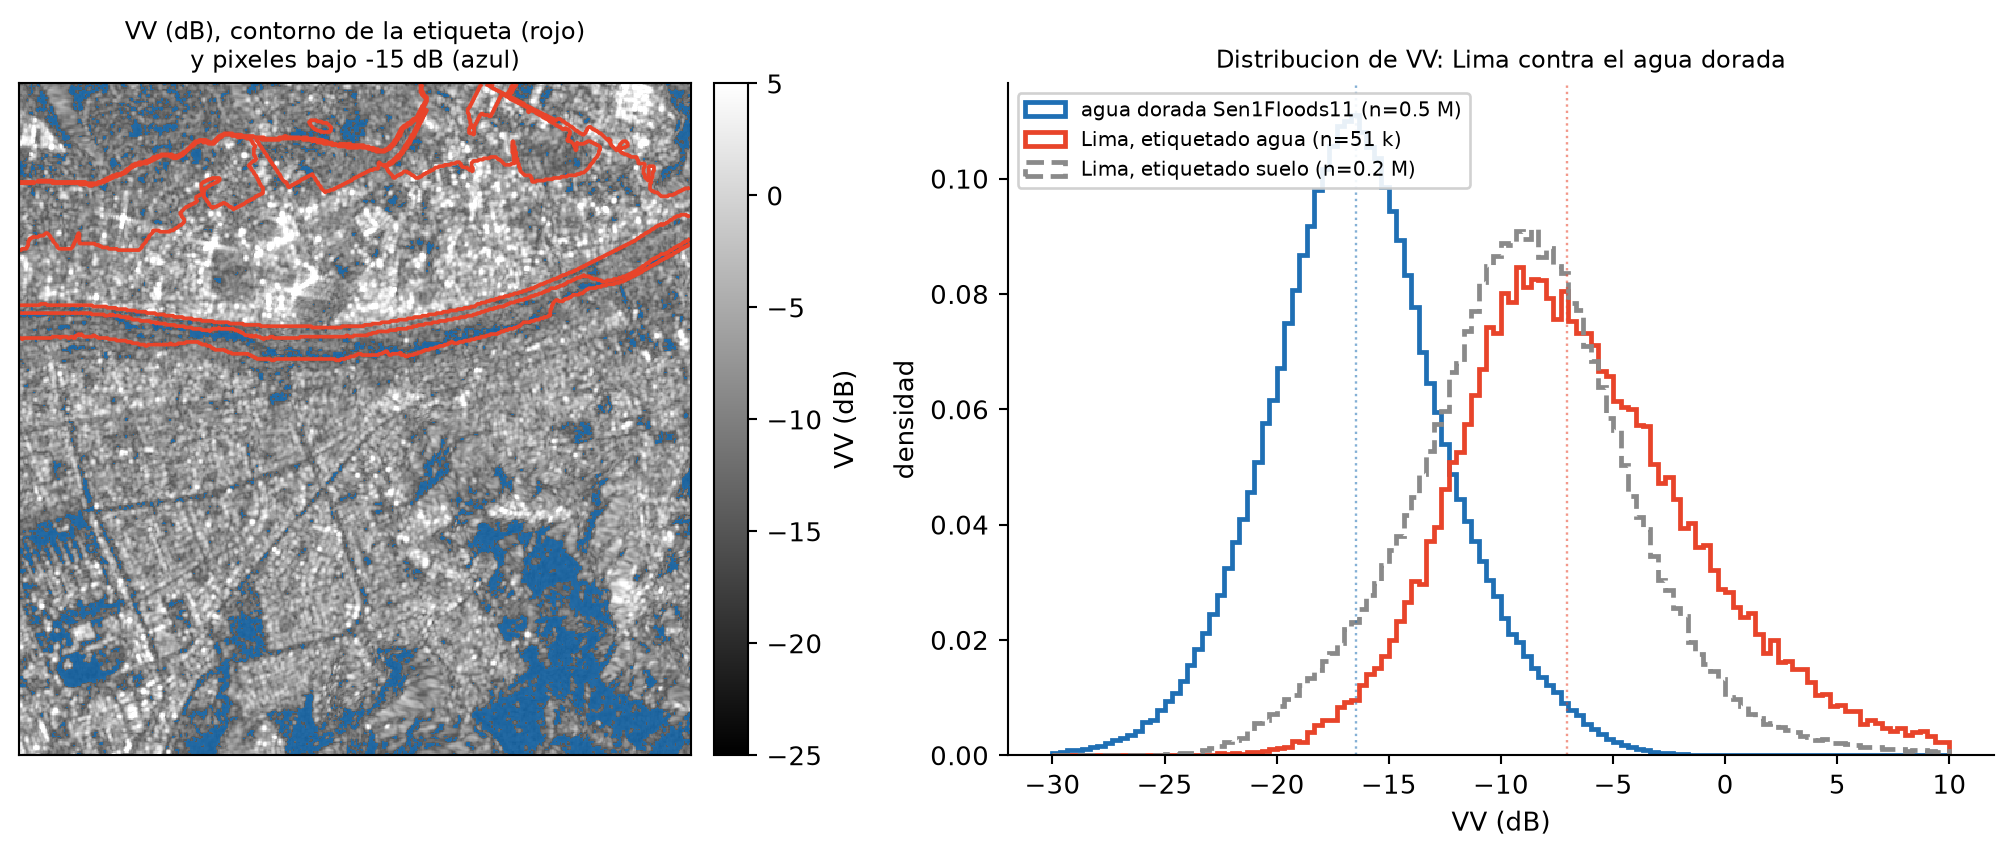
\includegraphics[width=0.74\textwidth]{figuras/etiqueta_lima.png}
\caption{\emph{Izquierda}: el contorno de la etiqueta (rojo) sigue el cauce (la
alineación es correcta), pero los píxeles oscuros (azul) están repartidos por
toda la escena y no dentro del contorno. \emph{Derecha}: las dos poblaciones de
Lima se superponen entre sí y ninguna cae donde cae el agua dorada. Lo etiquetado
agua es, si acaso, más brillante que lo etiquetado suelo.}
\label{fig:etiqueta}
\end{figure}

\paragraph{Firma de radar del cauce.}
El Cuadro~\ref{tab:firma} muestra que el \emph{cauce} es la capa más brillante de
todas, $-6.97$ dB, con apenas 1.4\% de píxeles oscuros. El Rímac de marzo de 2017 era un torrente de montaña turbulento
y cargado de sedimento en un cañón urbano, y una superficie rugosa retrodispersa
como suelo; lo que el radar ve negro es el agua \emph{lisa}. La confirmación está
en la última fila de Lima: \texttt{LakeresA}, lagunas de agua quieta, es la
única que se acerca al agua dorada. En el vocabulario de la
Sección~\ref{sec:fallos}, Lima es el modo 3, agua
brillante que se ve como suelo, extendido a un evento entero: ahí
pesaba el 2.5\% de los falsos negativos sobre 23.3 M de píxeles de Asia y África,
aquí domina la escena completa.

\paragraph{Tampoco la rescata la detección de cambio.}
Queda una salida: la detección de cambio, que es como Copernicus EMS mapea
inundaciones con SAR. Se bajó la escena del 5 de
marzo (mismo path, misma hora, doce días antes: mismo ángulo de incidencia
píxel a píxel) y se midió. Centrando la diferencia por escena, dentro de lo
etiquetado agua VV sube $+0.78$ dB mientras fuera no se mueve ($-0.01$).
Barriendo todos los umbrales de caída y quedándose con el mejor (elegido
viendo la respuesta, así que es una \emph{cota superior} de cualquier detector
por umbral global) el IoU máximo es 0.0242. El límite no es el modelo
de una fecha: el área señalada no se oscureció, se aclaró.

\paragraph{Qué queda en pie.}
No queda en pie leer el 0.0028 como medida de generalización: la
etiqueta marca la extensión máxima de la inundación, no la superficie de agua
visible en SAR que el modelo predice, así que comparar ambas mide el desacuerdo
entre dos definiciones. Bolivia sigue siendo el experimento de generalización
válido. Sobre la brecha de Lima pesan varias hipótesis: la definición de la
etiqueta (H1) y la firma turbulenta del cauce (H2), puestas a prueba con el
Cuadro~\ref{tab:firma} y la detección de cambio; el desbalance de clases, 1.01\%
frente a 9.51\% (H5), medido; y tres no medidas: el desfase temporal, el entorno
urbano y el distinto procesamiento radiométrico (H3, H4, H6). Sí queda en pie, y es un límite que conviene
documentar, que un producto de mapeo rápido de Copernicus no sirve como verdad de
terreno para SAR aunque describa la misma inundación, la misma semana y el mismo
lugar: ¿hasta dónde pudo llegar el agua? no es la pregunta que responde una
etiqueta de Sen1Floods11, ¿qué píxel es agua? La diferencia de medianas es de
7.3 dB.

\subsection{Fallos característicos del SAR (entregable 5)}
\label{sec:fallos}

Para separar los errores del sensor de los del modelo se construyen los
histogramas de VV condicionados a la verdad, uno para agua y uno
para suelo, sobre los 23.3 M de píxeles observados de prueba y Bolivia, y se
mide cuánto se solapan.

\begin{figure}[!htbp]
\centering
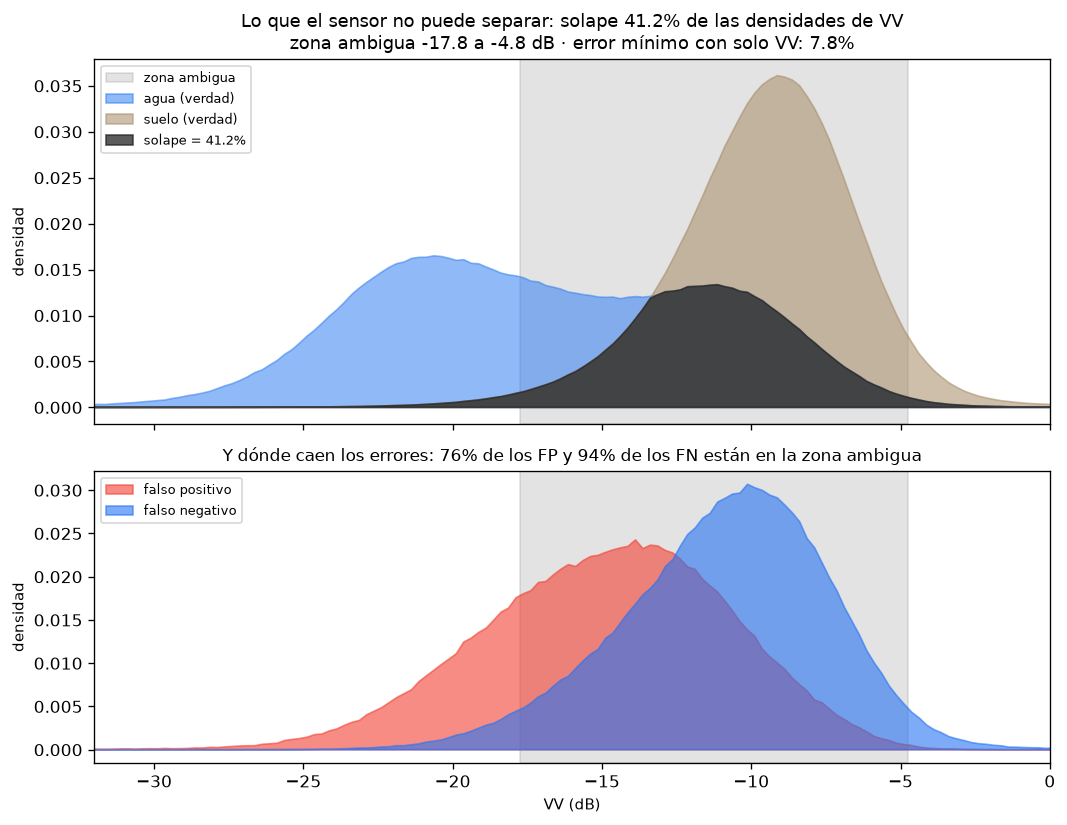
\includegraphics[width=0.62\textwidth]{figuras/separabilidad_vv.png}
\caption{\emph{Arriba}: densidades de VV condicionadas a la verdad. El área negra
es el solape, 41.2\% de la masa. La banda gris es la zona donde ninguna clase
domina el bin. \emph{Abajo}: dónde caen los errores del modelo. El 75.5\% de los
falsos positivos y el 94\% de los negativos están dentro de esa zona.}
\label{fig:separabilidad}
\end{figure}

\begin{table}[!htbp]
\centering
\caption{Los cuatro modos de fallo, con su peso medido. La zona ambigua va de
$-17.75$ a $-4.75$ dB.}
\label{tab:fallos}
\small
\begin{tabular}{lrrl}
\toprule
Modo & \% de los FP & \% de los FN & Zona de VV \\
\midrule
1 --- solape irreducible & 75.5\% & 94.0\% & ambigua \\
2 --- seco y liso se ve como agua (especular) & 24.3\% & --- & ambigua \\
3 --- agua brillante se ve como suelo (viento, doble rebote) & --- & 2.5\% & ambigua \\
4 --- el error cae donde su propia clase domina & 0.2\% & 3.5\% & \textbf{clara} \\
\midrule
\textbf{En zona ambigua de VV} & \textbf{99.8\%} & \textbf{96.5\%} & \\
\bottomrule
\end{tabular}
\end{table}

Las medianas lo dicen directo: los falsos positivos tienen VV $-14.6$ dB, mucho
más oscura que el suelo típico ($-9.4$), y los falsos negativos $-10.6$, mucho
más brillante que el agua típica ($-17.4$).

\begin{figure}[H]
\centering
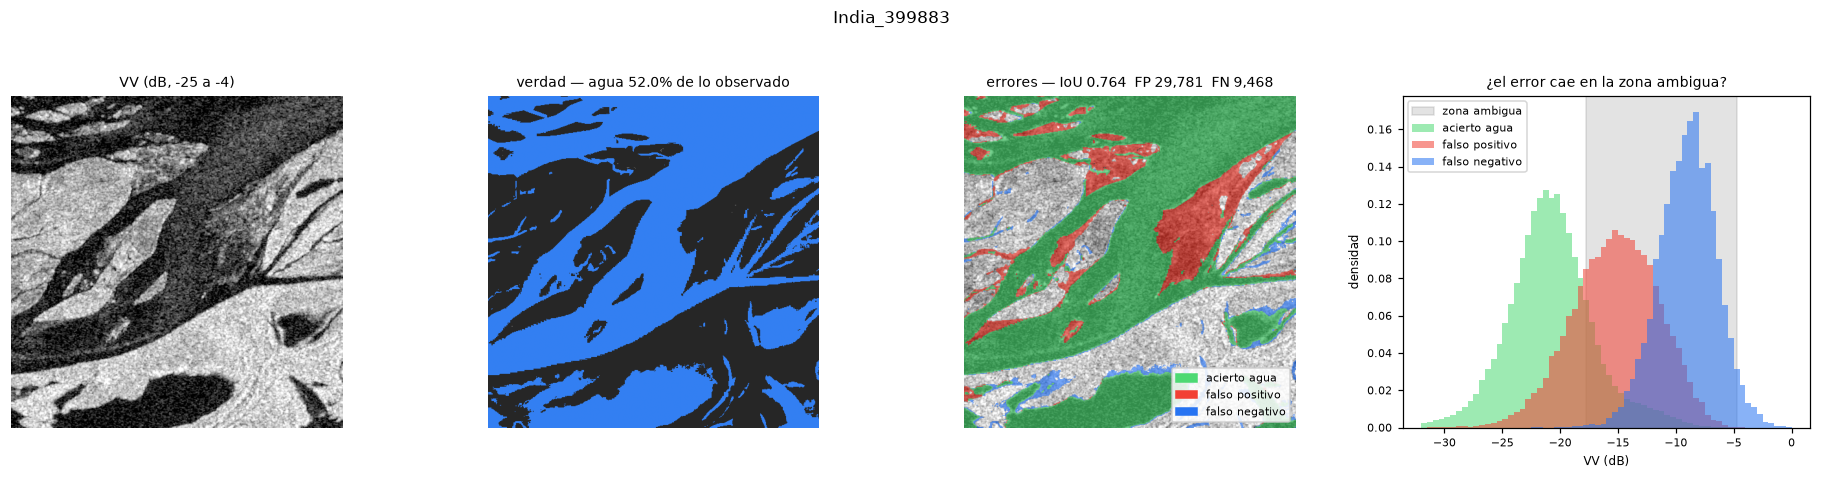
\includegraphics[width=0.60\textwidth]{figuras/modo1_solape.png}\\[1pt]
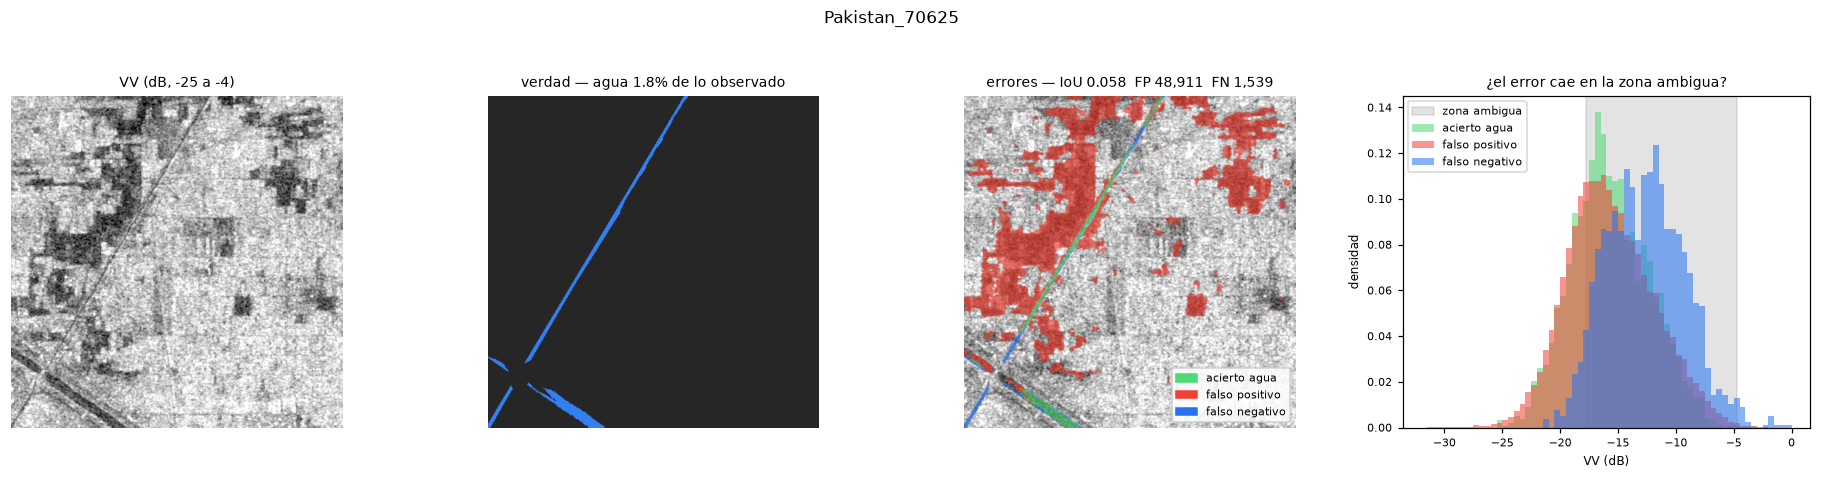
\includegraphics[width=0.60\textwidth]{figuras/modo2_especular.png}\\[1pt]
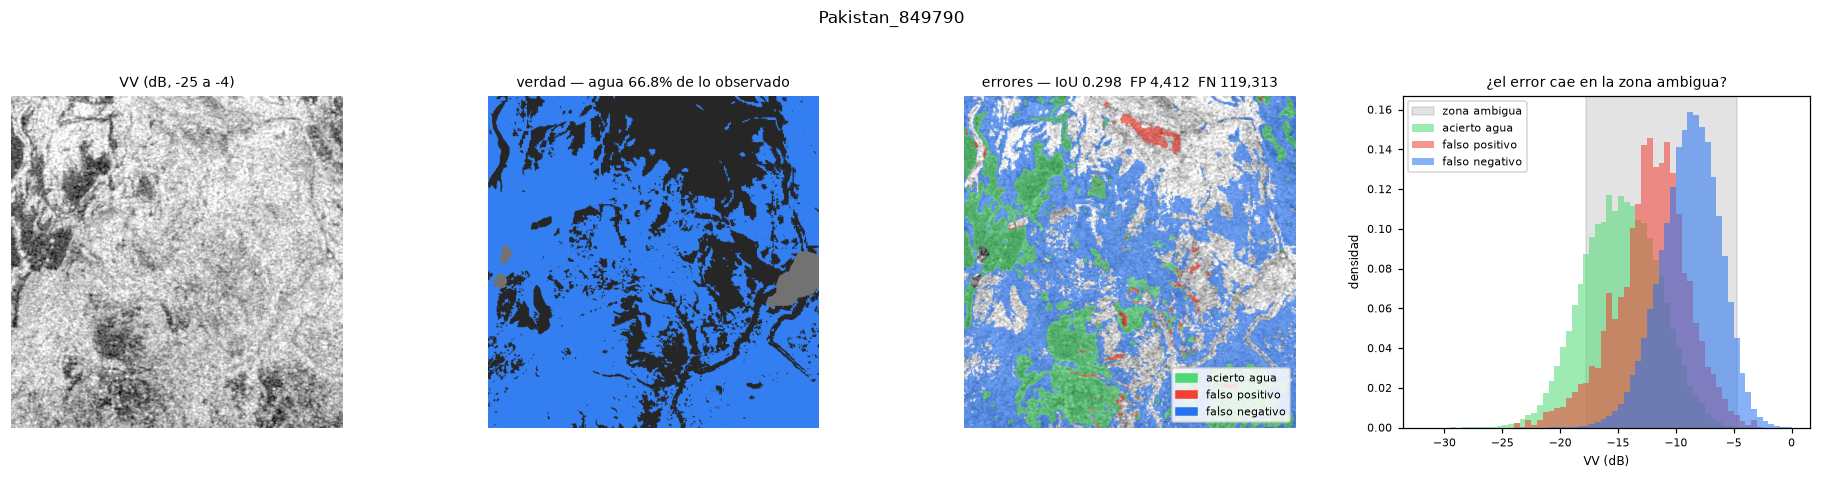
\includegraphics[width=0.60\textwidth]{figuras/modo3_agua_brillante.png}
\caption{Un ejemplo de cada modo de fallo del sensor; en cada fila: VV en dB, la
verdad, los errores (acierto de agua verde, falsos positivos rojo, falsos
negativos azul) y el histograma de VV con la zona ambigua sombreada.
\emph{Modo 1}, solape (\texttt{India\_399883}): el error cae en la zona gris.
\emph{Modo 2}, especular (\texttt{Pakistan\_70625}): campos secos marcados como
agua. \emph{Modo 3}, agua brillante como suelo (\texttt{Pakistan\_849790}): el
agua turbulenta se pierde como falso negativo.}
\label{fig:fallo}
\end{figure}

\paragraph{La comprobación de la cota.}
El error de Bayes mirando solo VV (con las proporciones reales, donde el
agua es el 12.8\% de los píxeles) es 7.81\%, y el modelo comete 4.83\%.
Está por debajo de la cota, que es lo que tiene que pasar: recibe VV \emph{y} VH
y además ve el contexto espacial.

\paragraph{La sombra de radar, un fallo que este conjunto no muestra.}
El enunciado nombra la sombra de radar entre los fallos característicos del SAR.
Es un artefacto geométrico: donde el relieve bloquea el pulso, la ladera opuesta
queda sin retorno y aparece negra, indistinguible del agua lisa. No figura entre
los cuatro modos cuantificados porque Sen1Floods11 cubre sobre todo llanuras y
deltas, donde la geometría apenas la produce, y porque las etiquetas doradas se
trazaron sobre escenas ya corregidas por terreno. Donde sí pesaría es en relieve
pronunciado como el cañón del Rímac, el mismo terreno de la región peruana
(Sección~\ref{sec:lima}): una sombra sobre la ladera se leería como agua y un
escorzo brillante escondería el cauce.

\paragraph{Sensibilidad a los umbrales.}
Barriendo 15 combinaciones de las dos constantes que definen la zona ambigua, la
fracción de error en esa zona va del 85.6\% al 100\% en los falsos positivos y
del 88.8\% al 99.1\% en los negativos: el reparto se mueve, la conclusión no.

\subsection{Fusión con Sentinel-2 (entregable 6, bono)}
\label{sec:fusion}

Si el radar no separa las clases, una banda óptica puede hacerlo.
Se entrena la misma U-Net tres veces (solo SAR, solo óptico, y los dos
fusionados) sobre los mismos chips, la misma partición y la misma semilla; lo
único que cambia son los canales de entrada. El modelo óptico usa las bandas B3,
B4, B8 y B11 más los índices NDWI y MNDWI. Los 446 chips dorados tienen las
tres piezas, así que no se pierde ninguno.

\begin{table}[!htbp]
\centering
\caption{Separación de cada capa óptica, con el mismo coeficiente de solape que
la Sección~\ref{sec:fallos} aplica a VV, sobre los 90 chips de prueba.}
\label{tab:separacion}
\small
\begin{tabular}{lrrr@{\qquad}lrrr}
\toprule
Capa & Agua & Suelo & Solape & Capa & Agua & Suelo & Solape \\
\midrule
Rojo B4 & 0.107 & 0.083 & 80.0\% & SWIR B11 & 0.038 & 0.198 & 13.9\% \\
Verde B3 & 0.128 & 0.107 & 70.9\% & NDWI & 0.165 & $-0.395$ & 11.3\% \\
NIR B8 & 0.092 & 0.273 & 15.2\% & \textbf{MNDWI} & \textbf{0.495} & $\mathbf{-0.285}$ & \textbf{9.4\%} \\
\midrule
\multicolumn{8}{l}{\emph{VV en dB, de referencia}: agua $-17.4$, suelo $-9.4$, solape \textbf{41.2\%}} \\
\bottomrule
\end{tabular}
\end{table}

MNDWI deja un 9.4\% de solape donde VV deja 41.2\%: lo reduce 4.4 veces.
Dos observaciones que la tabla deja ver: el
verde y el rojo por sí solos separan \emph{peor} que VV (70.9\% y 80.0\%), y el
salto está en el infrarrojo, donde la física lo pone.

\begin{table}[!htbp]
\centering
\caption{Bootstrap pareado sobre chips, 10\,000 remuestreos. Los 90 chips de
prueba se parten en 74 despejados y 16 nublados (más del 10\% de píxeles con
reflectancia en azul B2 $>$ 0.25).}
\label{tab:fusion}
\small
\begin{tabular}{llrcc}
\toprule
Comparación & Grupo & $\Delta$ IoU & IC95\% & ¿Significativa? \\
\midrule
\textbf{fusión vs.\ SAR} & todos & $+0.1690$ & $[+0.0910, +0.2538]$ & \textbf{sí} \\
 & despejados & $+0.1768$ & $[+0.0913, +0.2690]$ & \textbf{sí} \\
 & nublados & $+0.1220$ & $[+0.0186, +0.3405]$ & \textbf{sí} \\
\midrule
óptico vs.\ SAR & todos & $+0.1704$ & $[+0.0876, +0.2614]$ & sí \\
 & despejados & $+0.1832$ & $[+0.0937, +0.2808]$ & sí \\
 & \textbf{nublados} & $+0.0938$ & $\mathbf{[-0.0327, +0.3346]}$ & \textbf{no} \\
\midrule
fusión vs.\ óptico & todos & $-0.0013$ & $[-0.0122, +0.0093]$ & no \\
 & despejados & $-0.0063$ & $[-0.0168, +0.0007]$ & no \\
 & nublados & $+0.0282$ & $[-0.0020, +0.0567]$ & no \\
\bottomrule
\end{tabular}
\end{table}

Las IoU de prueba son 0.6808 (SAR), 0.8511 (óptico) y 0.8498 (fusión); la corrida
de SAR reproduce el 0.6808 del resto del informe.

El bono funciona, pero la fusión no le gana al óptico solo. La mejora sobre
el SAR es $+0.169$, pero la diferencia entre fusión y óptico es $-0.0013$ con el
intervalo cruzando cero: con cielo despejado el radar no aporta nada que el óptico
no tenga.

Con nubes, solo la ganancia de la fusión sigue siendo significativa. Fusión
contra óptico pasa de $-0.0063$ a $+0.0282$, con el intervalo rozando el cero por
dos milésimas: es donde la física dice que el radar tiene que aportar, pero con
16 chips nublados no se puede afirmar.

% ============================================================================
\section{Discusión crítica de las limitaciones}
% ============================================================================

\paragraph{Pocos chips nublados.}
Medido sobre los 90 de prueba: nubosidad mediana 0.2\%, 2 chips por
encima del 25\% y ninguno por encima del 50\%. El conjunto dorado se eligió
donde el óptico era etiquetable a mano, así que está sesgado hacia cielo
despejado. El régimen que motiva usar radar, óptico ciego y SAR solo, no tiene
aquí un solo chip.

\paragraph{Una sola región retenida.}
La inversión U-Net/Otsu en Bolivia es significativa, pero descansa en 15 chips de
una sola región. No se puede distinguir si el modelo falla por la región
\emph{boliviana} o por \emph{cualquier} región no vista, y el conjunto no ofrece
más regiones retenidas particionadas.

\paragraph{Techo de los chips débiles.}
El presupuesto está igualado en pasos, así que la comparación de \emph{qué datos}
es limpia; no se midió qué pasaría con 4\,412 chips y las 60 épocas completas,
diecisiete veces más cómputo. Una corrida así no superaría a la dorada, cuyo
techo es Otsu, pero eso es conjetura. Además, solo se probó concatenar las dos
fuentes; no se probó preentrenar con débiles y ajustar con dorados, ni ponderar
su pérdida. Las corridas de ablación usan una sola semilla y sin intervalo, así
que las diferencias menores a $\sim$0.02 no se interpretan.

\paragraph{Lima sin cifra de generalización.}
Queda sin responder cuánto cae el modelo en Lima: haría falta una delineación de
agua trazada sobre la propia escena SAR del 17 de marzo, que EMSN038 no provee.
La única región retenida con cifra válida sigue siendo Bolivia.

\paragraph{Variantes de arquitectura.}
Se ablacionó profundidad y pérdida, pero no se probaron las variantes que el
enunciado menciona (Attention U-Net \citep{oktay2018attention}, U-Net++
\citep{zhou2018unetpp}). Dado que la Sección~\ref{sec:fallos} ubica el 99.8\% de
los falsos positivos en la zona ambigua de VV, el retorno esperado de esa
búsqueda es bajo, aunque es una predicción, no un resultado medido. La cota de
Bayes de esa sección, además, se calculó solo sobre VV, no sobre VV y VH
conjuntos.

% ============================================================================
\section{Conclusiones}
% ============================================================================

Primero, más datos empeoran cuando la etiqueta la produjo el método que
se quiere superar: multiplicar el conjunto por diecisiete con chips de
umbralización baja la IoU de 0.681 a 0.587. No enseña a segmentar agua, enseña a
imitar a Otsu.

Segundo, el método clásico gana fuera de distribución, por $-0.088$ en
Bolivia y de forma significativa. La ventaja de Otsu es la que parecía su
limitación: recalcula su umbral en cada escena.

Tercero, casi todo el error cae donde VV es ambiguo, y eso condiciona
cómo leer lo demás: el 99.8\% de los falsos positivos cae donde las densidades de
agua y suelo se solapan, y el modelo opera por debajo de la cota de Bayes de una
sola banda. La fusión con Sentinel-2 sube la IoU a 0.850 porque MNDWI reduce ese
solape 4.4 veces, pero no le gana al óptico solo, y el régimen donde el radar
vuelve a ser necesario, el nublado, casi no está en el conjunto.

Cuarto, la etiqueta oficial de una inundación real no sirve como verdad
de terreno para SAR. En la región peruana el modelo cae a IoU 0.003, pero Otsu
cae con él, los píxeles oscuros abundan más fuera del agua declarada que dentro,
y entre el antes y el durante la zona señalada se \emph{aclara}. La delineación
de Copernicus marca la extensión máxima de la inundación, no la superficie de
agua visible en SAR.

La vía de mejora no es arquitectónica: hacen falta chips con nubosidad realista,
para saber si la fusión sobrevive al caso que motiva usar radar, y delineaciones
de agua trazadas sobre la propia escena SAR para medir generalización.

\section*{Reproducibilidad}
Todo se reproduce con \texttt{python pregunta2/ejecutar\_todo.py}, que encadena
las 20 etapas desde la descarga hasta este documento y salta las que ya tienen
artefacto. El repositorio incluye pruebas unitarias en \texttt{tests/}, que el
orquestador ejecuta, para el bootstrap pareado y el cálculo del solape.

\bibliographystyle{plainnat}
\bibliography{referencias}

\end{document}
